\section{Traffic Light Logic Preamble}
Before this report goes into the actual flows, explanation must be given in
regards to the traffic lights and how they were lit up. In the cases of flow 2
and flow 3, these lights are not shared by any other flows, so the flow 2 and 3
chips can directly control those lights with their Gr, Am, and Re outputs,
however in the case of the centre lights each set of lights would go green if
either of two specific flows were enabled, this problem was overcome by setting
up flows 5 and 6 to be ``masters'' of those lights and directly control them, with
input / light ``requests'' from flows 1 and 4 to each of them, figure \ref{fig:TL
flows red} on page \pageref{fig:TL flows red} illustrates which lights are
controlled by which flows.
\begin{figure*}
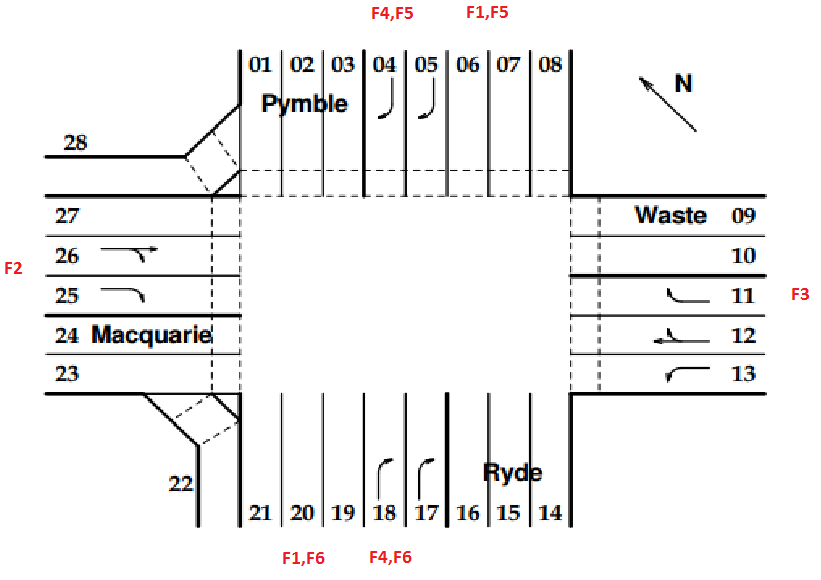
\includegraphics[width=\linewidth]{img/cXWehQ.png}
\caption{Traffic light flows for red lights}
\label{fig:TL flows red}
\end{figure*}

As can be seen, in the centre road both right and straight lights are controlled
by two flows exactly, flow 4 and flow 1 are on both sides, and flow 5 entirely
on one and flow 6 entirely on the other.

So what we did for flow 5 and 6 is gave them additional inputs, basically how
flows 4 and 1 would like the lights to be, these were called ``Buddy Left
Green'', ``Buddy left Amber" and so on, then within the equations for flow 5 and
6 (which will be shown later in more detail) the format is the following form
(with an example for flow 5):

\begin{lstlisting}[basicstyle=\ttfamily]
; Green left
GrL.D
  = (Flow 5 green eqn)
    + (Flow 1 green input)
; Green right
GrR.D
  = (Flow 5 green eqn)
    + (Flow 4 green input)

; Amber left
AmL.D
  = (Flow 5 amber eqn)
    + (Flow 1 amber input)
; Amber right
AmR.D
  = (Flow 5 amber eqn)
    + (Flow 4 amber input)

; Red left
ReL = /GrL*/AmL
; Red right 
ReR = /GrR*/AmR
\end{lstlisting}
Thus if flow 5 is green \textbf{both} sides will go green, and if flow 1 is on
the left will, and flow 4 the right.

\begin{figure*}
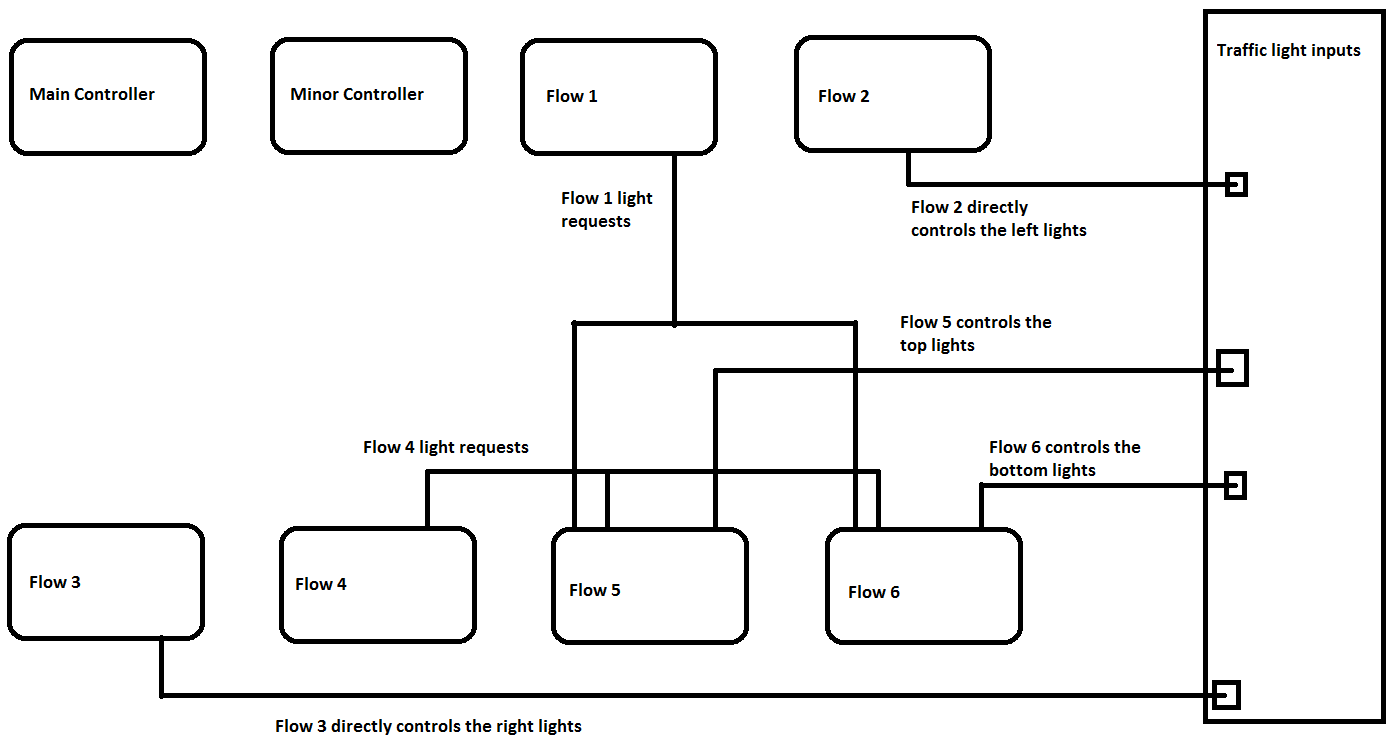
\includegraphics[width=\linewidth]{img/5Hvmk3.png}
\caption{Block diagram of light flow and control logic}
\label{fig:TLFlowControl}
\end{figure*}

The final point here is that flows 1 and 4 immediately pass on their requests to
flows 5 and 6, (I.E all equations in flows 1 and 4 for their lights have no
\texttt{.D} in them) however all other flows lights (with the exception of red
lights) have \texttt{.D}s in them, thus we designed the system to have the
lights be just one clock tick behind the chips. 